\documentclass{beamer}
\usepackage{beamerthemeshadow}
\usepackage[ngerman]{babel}
\usepackage[utf8]{inputenc}
\usetheme{Dresden}

\setbeamercovered{highly dynamic}

\begin{document}
  \title[CodeCover\hspace{105mm}\insertframenumber/\inserttotalframenumber]{CodeCover}
  %\title{CodeCover}
  \author{Michel Meyer und Manuel Schwarz}
  \date{\today}

  \begin{frame}
    \titlepage
  \end{frame}

  \begin{frame}
    \frametitle{Inhalt}
    \tableofcontents
  \end{frame}


  \section{Einleitung}
  \begin{frame}
    \frametitle{Motivation}
    \begin{itemize}[<+->]
      \item Softwarequalität erhöhen/verbessern
      \item Fehler schneller finden
      \item Code-Refactoring vereinfachen
      \item einfach zu bedienendes Tool
      \item evtl. IDE-Einbettung
      \item komfortable Bedienung
    \end{itemize}
  \end{frame}

  \section{Funktionsweise}
  \subsection{Tests}
  \begin{frame}\frametitle{Testarten}
  CodeCover deckt folgende Tests ab:
    \begin{itemize}[<+->]
      \item Bedingungsüberdeckung
      \item Zweigüberdeckung
      \item Schleifenüberdeckung
      \item Anweisungsüberdeckung
      \item Ternärer Operator Überdeckung
      \item Synchronisationsüberdeckung
    \end{itemize}
  \end{frame}

  \subsection{Technische Integration}
  \begin{frame}\frametitle{Benutzung}
    \begin{itemize}[<+->]
      \item Kommandozeile (Report erstellen)
      \item Eclipse (verschiedene Views + Report)
      \item Testfälle einfach erstellen und zusammenfassen
      \item Nutzen mit Ant
      \item Unterstützung von JUnit
    \end{itemize}
  \end{frame}

  \section{CodeCover allgemein}
  \subsection{Einsatzzweck}
  \begin{frame}\frametitle{White- bzw. Glass-Box Testing}
    \begin{itemize}[<+->]
      \item dynamisches Testverfahren
      \item strukturorientiert
      \item genauer: kontrollflussorientiert
      \item Prüfung direkt am Code im Gegensatz zum Blackbox Testing
      \item Ziel: Möglichst hohe Überdeckung
    \end{itemize}
  \end{frame}

  \subsection{Allgemeine Informationen}
  \begin{frame}\frametitle{Download und Toolinfos}
    \begin{itemize}[<+->]
      \item Quelle: kostenlos unter \texttt{codecover.org}
      \item letzte Version (Stand: März 2011): \texttt{CodeCover 1.0.1.2} (knapp 3 MB)
      \item Lizenz: Eclipse Public Licence (EPL)
      \item Plattformen: Kommandozeile (Linux, Windows, Mac OS) sowie Eclipse- und Ant-Integration
      \item Programmiersprachen: \texttt{Java} und \texttt{COBOL}
    \end{itemize}
  \end{frame}

  \subsection{Installation (Eclipse)}
  \begin{frame}
    \frametitle{Installation}
    \begin{columns}
      \begin{column}{4cm}
        \begin{itemize}
          \item \texttt{Eclipse} starten
          \item ``\texttt{Help}'' $\rightarrow$ ``\texttt{Install New Software\dots}''
          \item URL: \texttt{http://update.code\-cover.org/} eingeben
          \item \texttt{CodeCover} auswählen
        \end{itemize}
        \vspace{2cm}
      \end{column}
      \begin{column}{6cm}
        \begin{overprint}
          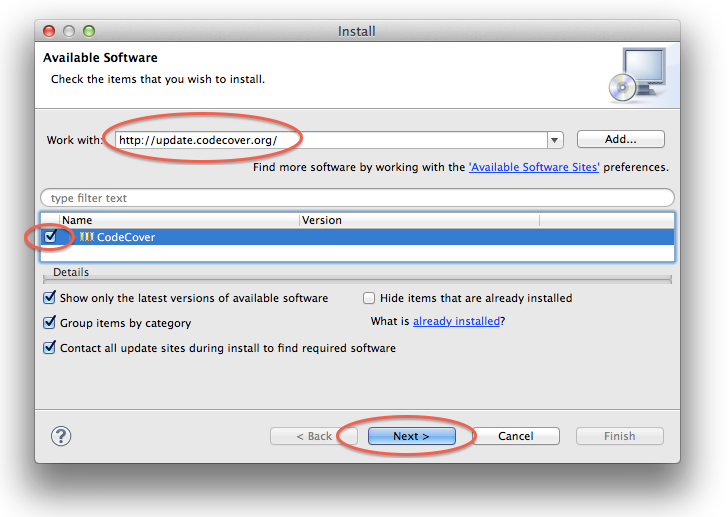
\includegraphics[width=7cm]{pictures/install.png}
        \end{overprint}
      \end{column}
    \end{columns}
  \end{frame}

  \begin{frame}
    \frametitle{CodeCover aktivieren}
    \begin{columns}
      \begin{column}{4cm}
        \begin{itemize}
          \item Rechtsklick auf gewünschtes Projekt
          \item \texttt{CodeCover} auswählen und aktivieren
          \item die gewünschten Kriterien auswählen
        \end{itemize}
        \vspace{2cm}
      \end{column}
      \begin{column}{6cm}
        \begin{overprint}
          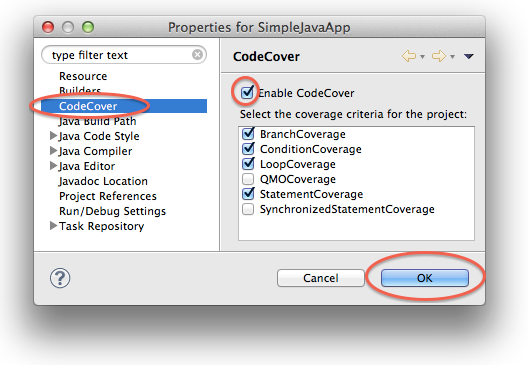
\includegraphics[width=6cm]{pictures/activate.png}
        \end{overprint}
      \end{column}
    \end{columns}
  \end{frame}

  \begin{frame}
    \frametitle{Zu prüfende Klassen auswählen}
    \begin{columns}
      \begin{column}{5cm}
        \begin{itemize}
          \item zu testende Klassen auswählen
          \item Rechtsklick $\rightarrow$ ``\texttt{Use For Coverage Measurement}''
        \end{itemize}
        \vspace{2cm}
      \end{column}
      \begin{column}{5cm}
        \begin{overprint}
          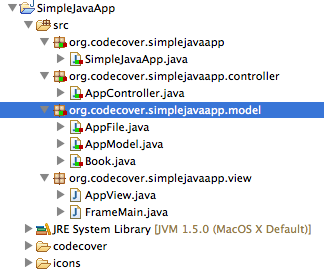
\includegraphics[width=4cm]{pictures/testclasses.png}
        \end{overprint}
      \end{column}
    \end{columns}
  \end{frame}

  \begin{frame}
    \frametitle{Ausführen}
    \begin{columns}
      \begin{column}{4cm}
        \begin{itemize}
          \item \texttt{Run} $\rightarrow$ \texttt{Run Configurations\dots}
          \item \texttt{Run with CodeCover} auswählen
          \item Ausführen
        \end{itemize}
        \vspace{2cm}
      \end{column}
      \begin{column}{6cm}
        \begin{overprint}
          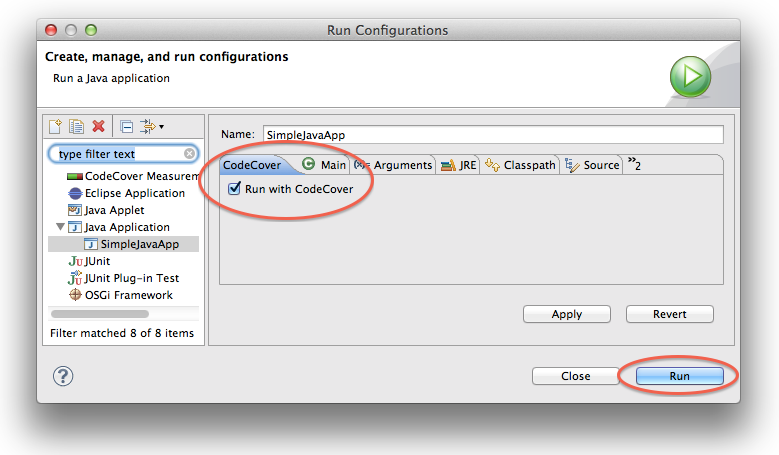
\includegraphics[width=7cm]{pictures/runconfigurations.png}
        \end{overprint}
      \end{column}
    \end{columns}
  \end{frame}


  \begin{frame}\frametitle{Farbkodierung}
    \begin{columns}
      \begin{column}{5cm}
        \begin{itemize}
          \item grün: komplette Abdeckung
          \item gelb: Teilabdeckung
          \item rot: wird nicht evaluiert
        \end{itemize}
        \vspace{1cm}
      \end{column}
      \begin{column}{5cm}
        \begin{overprint}
          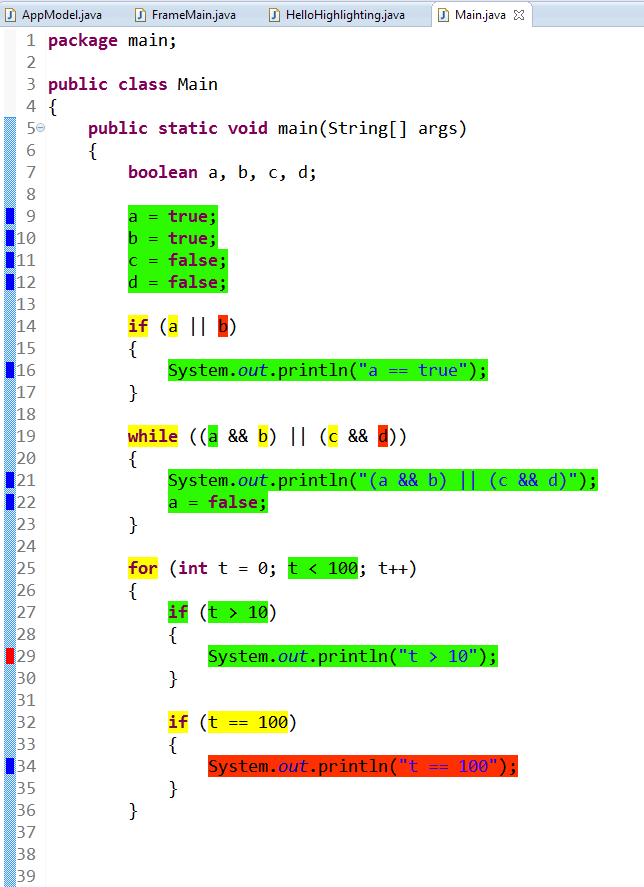
\includegraphics[height=65mm]{pictures/farben.png}
        \end{overprint}
      \end{column}
    \end{columns}
  \end{frame}

  \section{CodeCover Demo}
  \subsection{Kommandozeile}
  \begin{frame}\frametitle{einfaches Beispiel}
    \centering \Huge{DEMO}\\
  \end{frame}

%	\begin{frame}\frametitle{Instrument}
%    \begin{figure}%
%			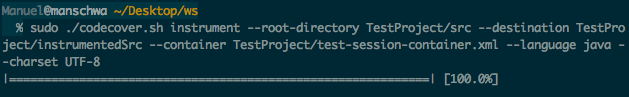
\includegraphics[width=\columnwidth]{pictures/demo_commandline/01_instrument.png}%
%			\caption{Source Code instrumentieren, d.h.\ zur Analyse vorbereiten.}%
%			\label{}%
%		\end{figure}
%  \end{frame}
%  
%  \begin{frame}\frametitle{Compile}
%    \begin{figure}%
%			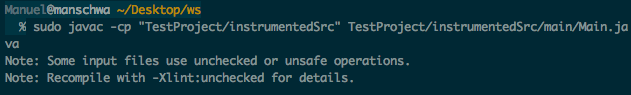
\includegraphics[width=\columnwidth]{pictures/demo_commandline/02_compile.png}%
%			\caption{Aufbereitete Dateien kompilieren\dots}%
%			\label{}%
%		\end{figure}
%  \end{frame}
%  
%  \begin{frame}\frametitle{Run}
%    \begin{figure}%
%			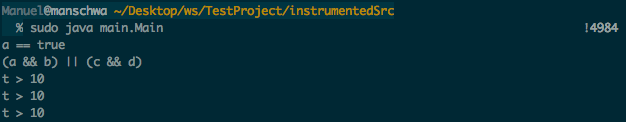
\includegraphics[width=\columnwidth]{pictures/demo_commandline/03_run.png}%
%			\caption{\dots und ausführen. Dabei wird eine clf-Datei erstellt, die die Ergebnisse beinhaltet und einen Testfall darstellt.}%
%			\label{}%
%		\end{figure}
%  \end{frame}
%  
%  \begin{frame}\frametitle{Analyze}
%    \begin{figure}%
%			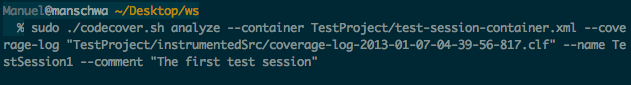
\includegraphics[width=\columnwidth]{pictures/demo_commandline/04_analyse.png}%
%			\caption{Die Ergebnisse werden analysiert und in eine xml-Datei eingefügt. Dabei kann ein \textit{merge} mehrerer clf-Dateien, also Testfälle, erfolgen.}%
%			\label{}%
%		\end{figure}
%  \end{frame}
%  
%  \begin{frame}\frametitle{Report}
%    \begin{figure}%
%			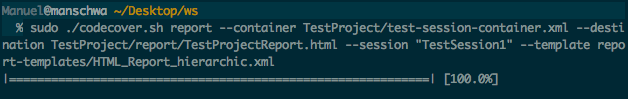
\includegraphics[width=\columnwidth]{pictures/demo_commandline/05_report.png}%
%			\caption{Schließlich wird ein Report auf Basis aller Ergebnisse in Form von html-Dateien erzeugt.}%
%			\label{}%
%		\end{figure}
%  \end{frame}
%  
%  \begin{frame}\frametitle{Report}
%    \begin{columns}
%      \begin{column}{5cm}
%        Darstellung der HTML-Datei mit den\\
%        \textit{Code Coverage}-Ergebnissen der Testfälle.
%        \vspace{1cm}
%      \end{column}
%      \begin{column}{5cm}
%        \begin{overprint}
%          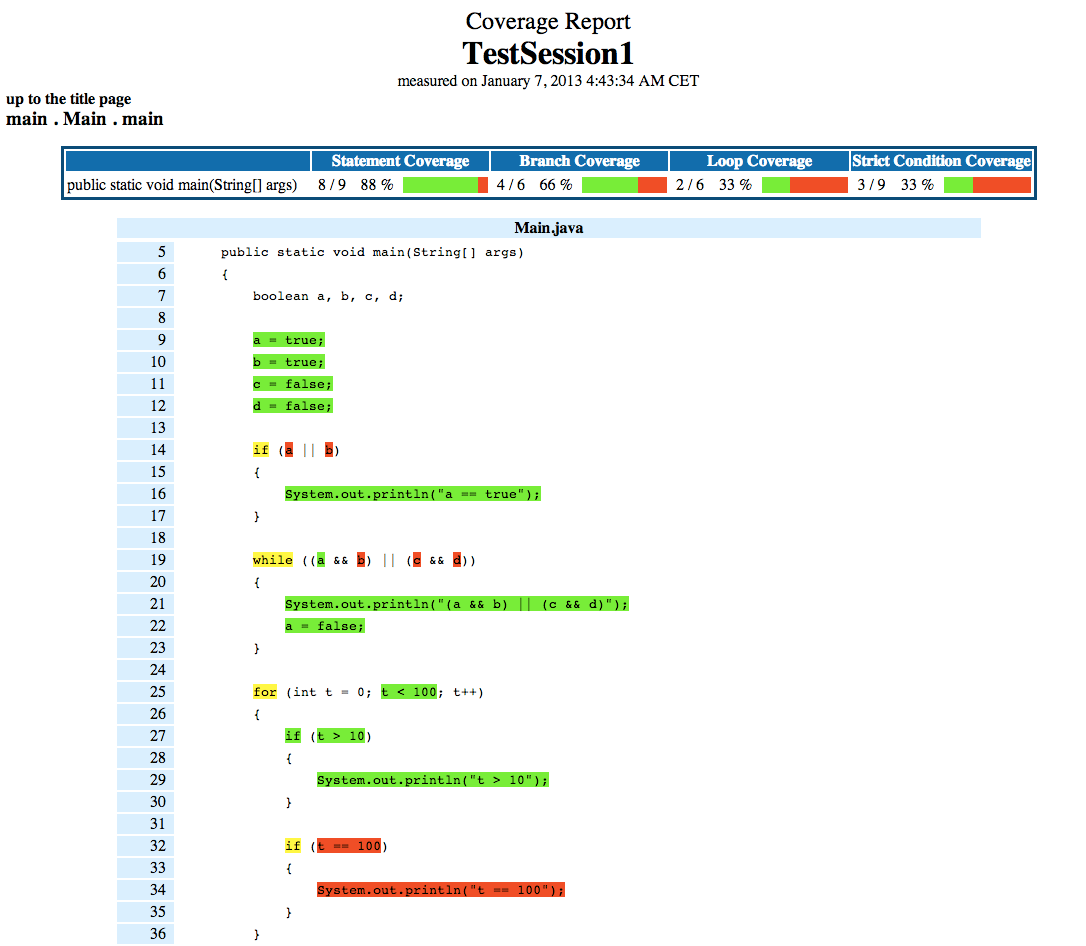
\includegraphics[height=45mm]{pictures/demo_commandline/06_report_html.png}
%        \end{overprint}
%      \end{column}
%    \end{columns}
%  \end{frame}

  \subsection{Eclipse}
  \begin{frame}\frametitle{komplexes Beispiel}
    \centering
    \Huge{DEMO}\\
    \centering
    \normalsize{\texttt{SimpleJavaApp}}\\
  \end{frame}

%  \begin{frame}\frametitle{Live Notification (1)}
%    Live Notification wird genutzt um verschiedene Testfälle zu generieren.\\
%    Notwendige VM Argumente:
%    \begin{block}{VM Argumente}
%      -Dcom.sun.management.jmxremote \\
%      -Dcom.sun.management.jmxremote.port=1234 \\
%      -Dcom.sun.management.jmxremote.ssl=false \\
%      -Dcom.sun.management.jmxremote.authenticate=false
%    \end{block}
%  \end{frame}
%
%  \begin{frame}\frametitle{Live Notification (2)}
%    \begin{columns}
%      \begin{column}{5cm}
%        \begin{itemize}
%          \item ``\texttt{Live Notification}''-View wählen
%          \item ``\texttt{localhost}'' als hostname und ``\texttt{1234}'' als port eintragen
%          \item Applikation starten
%          \item ``\texttt{connect}'' klicken
%          \item Testfälle generieren
%        \end{itemize}
%        \vspace{1cm}
%      \end{column}
%      \begin{column}{5cm}
%        \begin{overprint}
%          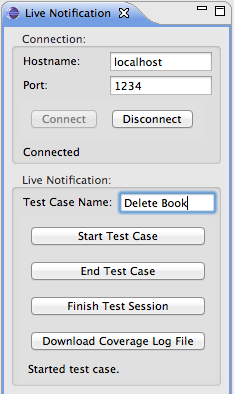
\includegraphics[height=50mm]{pictures/demo_eclipse/01_live_notification.png}
%        \end{overprint}
%      \end{column}
%    \end{columns}
%  \end{frame}
%
%  \begin{frame}\frametitle{Testfälle}
%    \begin{columns}
%      \begin{column}{5cm}
%        \begin{itemize}
%          \item Erzeugte Testfälle werden gespeichert
%          \item Auswahl treffen
%          \item View wählen und anzeigen
%        \end{itemize}
%        \vspace{1cm}
%      \end{column}
%      \begin{column}{5cm}
%        \begin{overprint}
%          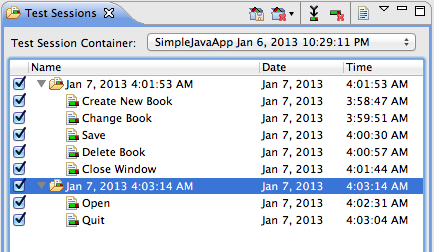
\includegraphics[width=4cm]{pictures/demo_eclipse/02_test_cases.png}
%        \end{overprint}
%      \end{column}
%    \end{columns}
%  \end{frame}
%
%  \begin{frame}\frametitle{Coverage View}
%    \begin{columns}
%      \begin{column}{5cm}
%        \begin{itemize}
%          \item Zeigt den Grad der jeweiligen Überdeckung an
%          \item hier: Anweisungsüberdeckung
%        \end{itemize}
%        \vspace{2cm}
%      \end{column}
%      \begin{column}{5cm}
%        \begin{overprint}
%          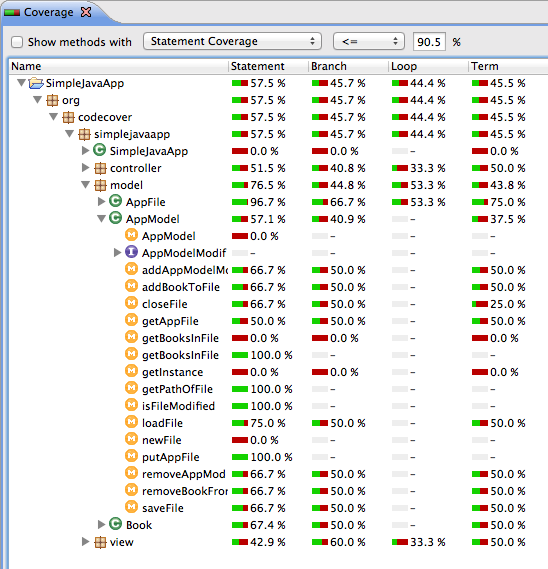
\includegraphics[height=6cm]{pictures/demo_eclipse/03_coverage_view.png}
%        \end{overprint}
%      \end{column}
%    \end{columns}
%  \end{frame}
%
%   \begin{frame}\frametitle{Correlation View}
%    \begin{columns}
%      \begin{column}{4cm}
%        \begin{itemize}
%          \item Zeigt an, wie stark unteschiedliche Testfälle miteinander korrelieren
%        \end{itemize}
%        \vspace{2cm}
%      \end{column}
%      \begin{column}{6cm}
%        \begin{overprint}
%          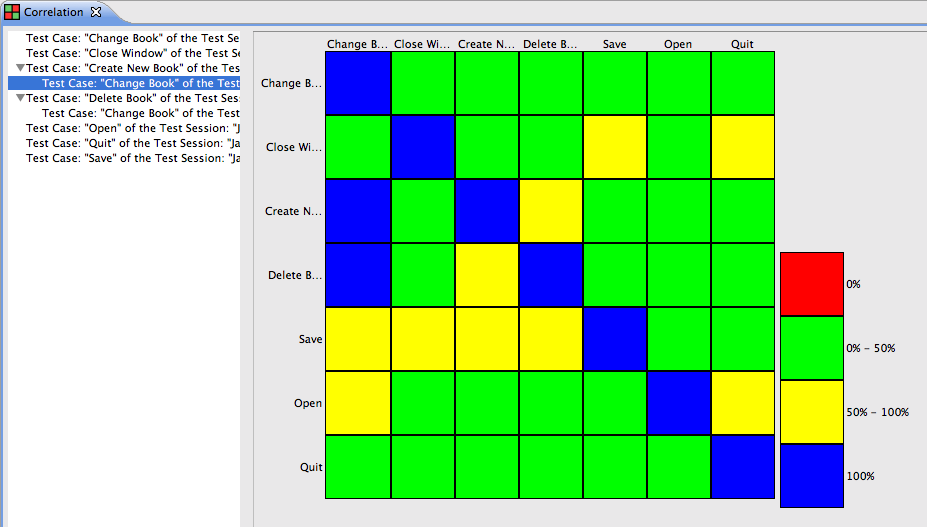
\includegraphics[width=7cm]{pictures/demo_eclipse/04_correlation_view.png}
%        \end{overprint}
%      \end{column}
%    \end{columns}
%  \end{frame}


  \section{Fazit}
  \begin{frame}\frametitle{Zusammenfassung und Fazit}
    \begin{itemize}[<+->]
      \item gute Eclipse-Integration
      \item einfaches Generieren und Zusammenfassen von Testfällen
      \item verschiedene nützliche Views in Eclipse
      \item keine Weiterentwicklung seit fast 2 Jahren
      \item nur \texttt{Java} und \texttt{COBOL} werden unterstützt
      \item evtl. Alternativen suchen
    \end{itemize}
  \end{frame}



\end{document}
